% \glsresetall
\chapter{Webpack Module Federation} % Main chapter title
\label{Chapter5}

\lhead{Chapter 5. \emph{Webpack Module Federation}}

A rather new technology on the market is the \textbf{Webpack 5 Module Federation (WMF)}. The Module Federation was part of Webpack's 5th version, released on October 10, 2020. It added features which improved its usage for developing micro frontends.\cite{wmf_concepts}
The way it does that, is via modularizing self-compiled code parts and publishing them for integration by other modules. This published modules are called \textbf{remotes} whereas the integrating modules are called \textbf{hosts}. 
\textbf{Hosts} refer to \textbf{remotes} under a configured name. This name is not actually known to the \textbf{host} during the compile time, but is first resolved at runtime.
The self-compiled \textbf{remotes} can be anything, a micro frontend or some sort of utility script. This way the Module Federation provides a way to avoid external or manual script loading and instead gives opportunities to automatically lazy load necessary code blocks during runtime.\cite{wmf_concepts}
The usage of the WMF is tied to the Webpack bundler, since the necessary configuration is done in the \texttt{webpack.config.js}. This restriction is applied to every \textbf{remote} in the WMF landscape, not only to the \texttt{host}.

WMF provides means to solve the issue, described in this thesis. First a short introduction of WMF is given, then the shared dependency feature is explained.
It is mentioned, that WMF can be used in combination with most of the common UI frameworks. But since the implementation for this thesis was done with Angular, the further examples and explanations will be Angular-based.

\section{Enabling the Module Federation}

Prior to introducing the usage of the Module Federation, it is necessary to introduce Webpack itself first, as it is a mandatory feature for using the Module Federation. The documentations of popular UI frameworks, like React, VueJS or Angular, imply that Webpack is used by default, but this can customized by a developer is needed \cite{webpack_angular}\cite{webpack_react}\cite{webpack_vue}.

To change the default configurations, the necessary \texttt{webpack.config.js} file has to be enabled first.
In case of Angular, two dependencies have to be installed, using e.g. the Angular CLI. By enabling the Webpack configuration file, the features of the Module Federation are enabled, too. The command used for this is shown in \ref{list:angluar_wmf_command}. 

\begin{lstlisting}[language=Bash, caption=Angular CLI console command to enable Module Federation in an Angular project, label=list:angluar_wmf_command,  xleftmargin=.0\textwidth, xrightmargin=.0\textwidth]
	ng add @angular-architects/module-federation --project name --port port
\end{lstlisting}

These commands are necessary, since the CLI protects the Webpack configuration from access. The \texttt{@angular-architects/module-federation} package provides a custom builder, via which this access restriction is lifted.
After installing this dependency in an Angular project, a \texttt{webpack.config.js} will appear on root level of the corresponding project.\cite{wmf_angular_dependency_install}
This dependency has to be added in each \textbf{remote} or \textbf{host} of the WMF landscape, to enable the Module Federation in those projects.

After the enabling, the necessary configuration can be applied to the \texttt{webpack.config.js} file. The \textbf{remotes} publish their modules and \textbf{hosts} consume them. 

\section{Shared dependency feature}

The shared dependency feature of WMF, is a way to solve the issue of redundant libraries in its landscapes.
This feature is enabled and configured, as well as the rest of the WMF, via the \texttt{webpack.config.js}. When configuring the components of the landscape, it is possible to define a section where shared dependencies are described. These dependencies can be defined in different ways. For instance, it is possible to define a strict version of the dependency, which would result in the framework loading this specific version. Another option can be, a less restricted dependency definition, which results in the framework, loading of highest major version available. WMF is able to distinguish between major versions of the dependencies, shared in its landscapes. If not configured otherwise, it automatically picks the highest major version and applies it to the sharing modules. 

\begin{lstlisting}[language=JavaScript, caption=Example of sharing dependencies configured in the \texttt{webpack.config.js}, label=list:shared_mapping_wmf,  xleftmargin=.0\textwidth, xrightmargin=.0\textwidth]
	shared: share({
		"@angular/core": { 
			singleton: true, 
			strictVersion: false, 
			requiredVersion: '12.2.0' 
		},
		"@angular/common": { 
			singleton: true, 
			strictVersion: false, 
			requiredVersion: '12.2.0' 
		},
		"@fundamental-ngx/core": { 
			singleton: true, 
			strictVersion: false, 
			requiredVersion: '0.33.0-rc.214' 
		},
		
		...sharedMappings.getDescriptors()
	})
\end{lstlisting}

Listing \ref{list:shared_mapping_wmf} is an example of how to share libraries in a restrictive way. To provide a less restricted configuration, a simple array of the shared dependency names suffices. But to ensure a redundant free landscape, these restrictions are necessary. Each configuration property will be explained below.

\begin{itemize}
	\item \texttt{singleton} - This property defines, if the dependency should be able to be loaded more than once in different versions or not. If set to \texttt{true}, WMF will automatically pick the highest version of a major release of this dependency available and distribute it to the \textbf{remotes}.\cite{wmf_version_mismatch}
	
	\item \texttt{strictVersion} - This property defines, if the dependency requires a specific version to work. If set to \texttt{true}, WMF will load the required version, even if another dependency mapping with the same name is present. This can lead to conflicts with the \texttt{singleton} property, if configured poorly.
	
	\item \texttt{requiredVersion} - This property defines, the required version of the dependency. When working with a package manager (e.g. NPM), this version has to be aligned with the locally installed version of the dependency. If the \texttt{strictVersion} property is set to \texttt{false}, this property defines the minimum version for the micro frontend. 
	
	It has to be mentioned, that WMF is does not apply one dependency to all remotes if different major releases are configured for them. If a higher version of the same major release is available, it will only be loaded for the modules with the same major release configured. Modules with a lower or higher, major release required, are not affected by it \cite{wmf_multi_versions}. This aspect is explained further below.
\end{itemize}

Now, when it comes to sharing the dependencies inside the micro frontend landscape, each \textbf{remote} has to participate. That means each micro frontend has to define its required dependencies in their respective versions. Additionally, it has to be mentioned that the micro frontends themselves have to use dynamic imports when importing shared dependencies. Through the asynchronous behavior of the import, Webpack has time to pick the correct version of the dependency inside the landscape.\cite{wmf_concepts}
Analyzing this statement in combination with the information taken from \ref{list:shared_mapping_wmf}, it becomes obvious that multiple versions of the same framework can exist in a landscape. 

\section{Multi-version landscapes in WMF}

Figure \ref{fig:wmf_multiversions} illustrates the case, of how WMF handles a multi-version landscape.

\begin{figure}[!h]
	\centering
	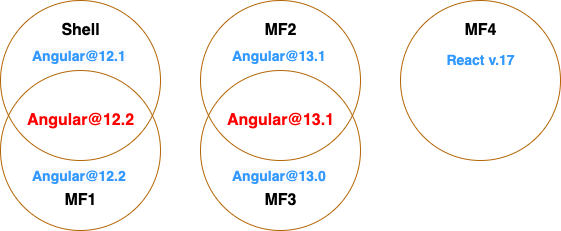
\includegraphics[width=0.7\textwidth]{Figures/multi_version_diagramm.drawio.png}
	\caption{WMF way of handling multi-versions}
	\label{fig:wmf_multiversions}
\end{figure}

As it can be seen, WMF always picks the latest major release, assuming the respective micro frontends have a similar configuration as shown in listing \ref{list:shared_mapping_wmf} applied. If, for instance, \textbf{MF3} has the \texttt{strictVersion} property set to \texttt{true}, for a dependency, it would cause the loading this library, too. Even if, it is already present in a different version.

There are side effects to sharing the same dependency over the whole micro frontend landscape. One of which is the increase in bundle sizes, since every \textbf{remote} bundles its local dependencies. WMF then, picks the ones to serve during the runtime of the landscape.
This impact has a trade-off tough. Returning users can benefit from cached dependencies, since the same bundles are reused, loading the site.\cite{wmf_multi_versions}

Therefore, WMF is able to reduce redundant libraries in micro frontend landscapes and additionally supports multi-version environments, via the shared dependency feature.